\chapter{Implementazione}
\label{ch:implementazione}

In questa sezione verranno descritte le scelte implementative ed i componenti impiegati che hanno consentito la realizzazione di una rete in rispetto delle specifiche definite nel capitolo di \textit{\nameref{ch:progettazione}}.\\ 
Il seguente lavoro di tesi ha previsto la definizione di due approcci così strutturati: nel primo si è utilizzata solo la tecnologia \texttt{Bluetooth Mesh}, mentre nel secondo è stata integrato lo standard \texttt{802.11} come tecnologia di supporto.\\
In entrambi gli approcci sono stati utilizzati quattro dispositivi ESP32 con i seguenti ruoli: 

\begin{itemize}
    \item un dispositivo \textit{client} il cui compito è quello di inviare i messaggi all'interno della rete con una frequenza indicata in input dall'utente, avvalendosi di uno script \texttt{Python}. In più, è in continua comunicazione, tramite porta seriale, con il PC per assicurare la definizione di un file di log. 
    
    \item due dispositivi aventi il ruolo di \textit{relay}. Sfruttati solo con la tecnologia Bluetooth Mesh, poiché con la tecnologia 802.11 è stato necessario introdurre un dispositivo esterno, con il ruolo di \textit{router}.
    
    \item un dispositivo \textit{server} avente il compito di ricevere dei messaggi precedentemente inviati dal client, attuare il cambiando di stato comunicato e confermare tale ricezione utilizzando la medesima tecnologia del messaggio ricevuto.
\end{itemize}

\noindent Per garantire la creazione della rete mesh è stato necessario l'utilizzo di un dispositivo in grado sia di supportare un'applicazione di provisioning sia in grado di eseguire le operazioni di routing per la tecnologia Wi-Fi. Per soddisfare entrambe queste richieste è stato adottato uno smartphone con supporto a Bluetooth 5. Oltre a tale dispositivo è stato necessario l'impiego di un PC non solo per programmare i vari nodi attraverso il framework \texttt{ESP-IDF} ma anche per consentire la comunicazione con il nodo client, necessaria per comunicare il comportamento da assumere e per ricevere e archiviare gli eventi innescati su tale nodo durante l'esecuzione del test.

\section{Dispositivi}
Come anticipato all'inizio del capitolo, per la realizzazione del seguente progetto di tesi sono stati coinvolti i seguenti dispositivi. Di seguito una breve descrizione.
\subsection{ESP32}
% http://esp32.net/
% https://en.wikipedia.org/wiki/ESP32
% https://www.espressif.com/en/products/hardware/esp32/overview
% http://www.lucadentella.it/2016/12/03/esp32-1-introduzione/
% https://www.zerozone.it/tecnologia-privacy-e-sicurezza/primi-esperimenti-di-iot-con-i-moduli-esp32/13230
Il dispositivo ESP32 indica una serie di microcontrollori a basso costo e a bassa potenza il cui chip è in grado di supportare le tecnologie di comunicazione \texttt{Wi-Fi} e \texttt{dual-mode Bluetooth}. \\
A settembre 2016 Espressif Systems (una società cinese con sede a Shangai) ha annunciato e reso disponibile il chip successore ad ESP8266, chiamato appunto ESP32, il quale ha introdotto un numero maggiore di pin GPIO, la presenza della connettività Bluetooth, un sensore touch e maggiore memoria.\\ 
Il nucleo di questi nuovi dispositivi è costituito da un microprocessore Tensilica Xtensa LX6 a 32-bit nelle varianti single-core o dual-core, in grado di operare con una frequenza comprese tra 80 e 240 MHz.\\
L'integrazione di Bluetooth, Bluetooth Low Energy e Wi-Fi garantiscono  l'impiego in una vasta gamma di scenari sopratutto in contesti IoT. Il Wi-Fi garantisce la copertura di una zona piuttosto ampia ed una diretta connessione ad Internet tramite l'utilizzo di un router Wi-Fi, mentre il Bluetooth consente lo scambio di informazioni su un'area nettamente inferiore ma con consumi nettamente più bassi. 
Il ridotto consumo energetico è garantito grazie a specifiche funzioni, tra cui la gestione dei clock e il ridimensionamento dinamico della potenza.\\

\noindent Una scheda di sviluppo dotata di chip ESP32, per poter funzionare necessita di alcuni componenti esterni a tale chip: una memoria flash (in cui sono memorizzati il firmware e i dati), un modulo per il Real Time Clock (RTC), un'antenna e alcuni componenti passivi.\\
Sul mercato, si trovano diverse tipologie di circuiti stampati personalizzati con su integrato il chip ESP32. Oltre al chip tale board sono dotate di appositi moduli tra l'altro estendibili, grazie al numero elevato di PIN I/O i quali consentono di sviluppare progetti sempre più complessi.\\
Tali schede montano uno stabilizzatore di tensione che permette la corretta alimentazione dei moduli, il convertitore \texttt{USB-UART} e i tasti \texttt{RESET} e \texttt{FLASH} che semplificano il processo di programmazione. \\
Esistono diversi firmware per gestire questi chip, quello utilizzato in tale circostanza risulta essere il firmware ufficiale, ovvero quello rilasciato da \texttt{Espressif} e consente la comunicazione con il modulo attraverso dei comandi AT. % comandi AT -> particolari stringhe utilizzare per comunicare con diversi dispositivi elettronici.
Un firmware alternativo, di tutto rilievo, è chiamato NodeMCU ed è basato su Lua, un linguaggio di programmazione dinamico e veloce simile al Python.\\

\noindent In base alle necessità richieste dal seguente progetto, ovvero poter utilizzare contemporaneamente lo stack Wi-Fi e BLE, sono stati utilizzati dispositivi \textit{ESP32-WROVER} dotati di una memoria supplementare rispetto ai dispositivi \textit{ESP32-WROOM} maggiormente diffusi.\\
Nello specifico ESP32-WROVER presenta una memoria Flash SPI di 4 MB ed una Pseudo Static RAM (PSRAM) aggiuntiva di 8 MB.
\begin{figure}[!ht]
    \centering
    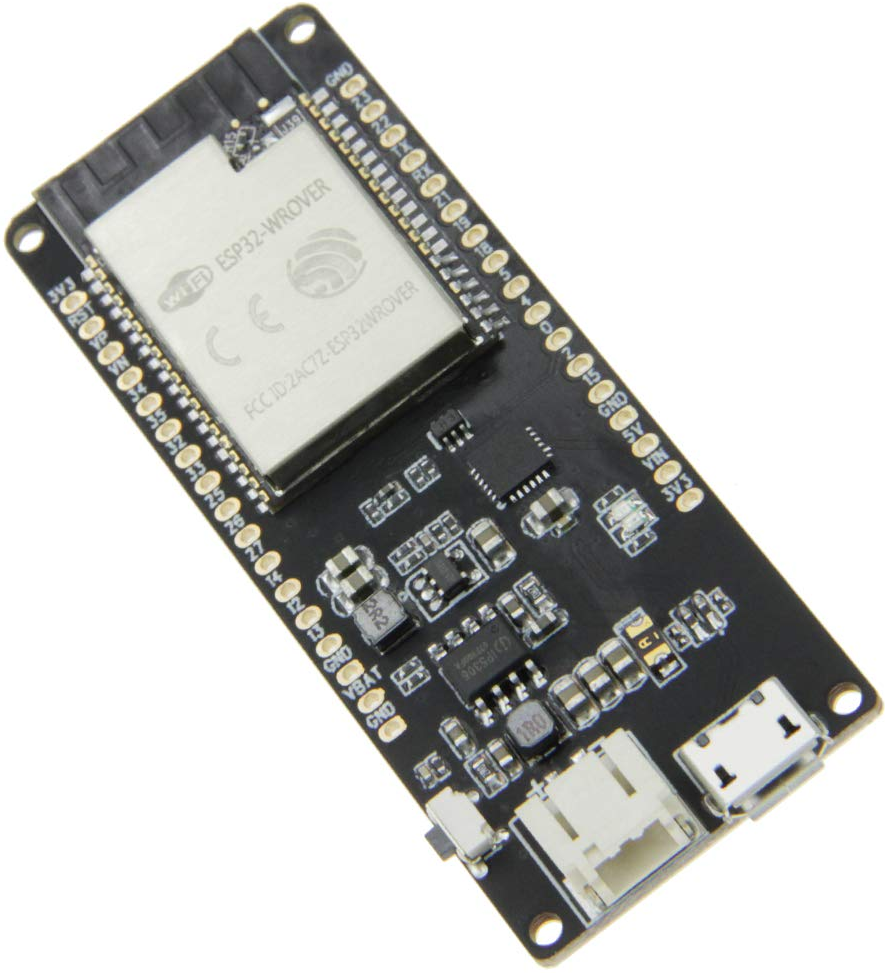
\includegraphics[width = 0.5\textwidth]{images/esp32_wrover.png}
    \caption{ESP32 WROVER}
    \label{fig:esp32_wrover}
\end{figure}

\subsubsection{Ambiente di sviluppo}
Per sviluppare un applicativo eseguibile su tali dispositivi la scelta può ricadere su diversi ambienti di sviluppo. Di seguito una rapida descrizione di \texttt{Arduino IDE}, molto semplice da utilizzare, e il framework messo a disposizione da Espressif (\texttt{ESP-IDF}) utilizzato in questo contesto applicativo.\\
Arduino IDE è un framework open-source che consente di avere un approccio piuttosto semplice per la programmazione dei moduli e per l'upload del codice sulle board compatibili con l'IDE. Prima di procedere con la compilazione del codice da copiare sulla propria board, è fondamentale aggiungere le apposite librerie al fine di rendere la board compatibile, nel caso in cui non lo era.\\
% http://wiring.org.co/
Utilizzando Arduino IDE è possibile creare un applicativo (sketch) per il proprio microcontrollore sfruttando una libreria software del progetto \textit{Wiring}. Wiring oltre ad essere una piattaforma di prototipazione open-source, fornisce delle regole per la strutturazione del codice relativo alle comuni procedure di input e di output utilizzando un linguaggio di programmazione derivato dal \texttt{C++}.\\
% https://en.wikipedia.org/wiki/Arduino_IDE
Il codice scritto dall'utente richiede solo due funzioni base: 
\begin{itemize}
    \item \textit{setup}: una funzione eseguita solo una volta, all'avvio dello sketch e può essere usata per definire le impostazioni iniziali dell'ambiente.
    \item \textit{loop}: una funzione invocata continuamente, finché la board non viene spenta. Tale funzione descrive il comportamento che dovrà assumere il dispositivo durante il suo periodo di attività.
\end{itemize}
Una volta creato lo sketch e configurato l'IDE per supportare la board in possesso è possibile procedere con l'upload del codice e interagire (attraverso la seriale) con l'applicativo grazie agli strumenti messi a disposizione da Arduino IDE.\\

% http://www.lucadentella.it/2016/12/12/esp32-2-lambiente-di-sviluppo/
% https://github.com/espressif/esp-idf
\noindent L'alternativa ad Arduino IDE per programmare i chip in dotazione è Espressif IoT Development Framework (ESP-IDF), rilasciata proprio dalla casa produttrice e indicata come il framework ufficiale di prototipazione per tali board.
Come il tool precedente, anche esso risulta essere open-source e cross-platform (disponibile per Windows, Linux e Mac OS), anche se il suo utilizzo è sensibilmente più complicato e qualsiasi operazione deve essere svolta tramite console.\\
Il framework ESP-IDF è reperibile presso il repository ufficiale \href{https://github.com/espressif/esp-idf}{GitHub} di Espressif: \url{https://github.com/espressif/esp-idf}. Dopo aver scaricato, installato e configurato l'intero ambiente (variabili d'ambiente, toolchain per compilare il codice, tools per la creazione di un'applicazione) e possibile finalmente implementare un'applicazione eseguibile da un dispositivo Espressif.\\
Come indicato dalla documentazione ufficiale, le operazione relative ad ogni progetto da eseguire sui predetti dispositivi sono indicate in seguito e prevedono sempre l'utilizzo dell'istruzione \texttt{idf.py}. Le seguenti istruzioni dovranno essere eseguite solo dopo essersi posizionati nella directory del progetto da gestire.
\renewcommand{\theenumi}{\roman{enumi}}
\begin{enumerate}
    \item \texttt{idf.py menuconfig}: consente la configurazione del progetto in base al dispositivo che dovrà eseguirlo. Con il seguente comando si ottiene un menu che consente di specificare determinati parametri riguardanti ``\texttt{SDK tool configuration}'', ``\texttt{Bootloader config}'', ``\texttt{Serial flasher config}'', ``\texttt{Partition Table}'', per citarne alcuni. \\
    All'interno di tale menu, oltre alle voci menzionate, è possibile definire una voce ``\texttt{Example Configuration}'' che, attraverso un'estensione basata su Python (kconfiglib), fornisce un meccanismo di configurazione del progetto in fase di compilazione. Il file \texttt{kconfig} consente all'utente di specificare apposite informazioni in base al dispositivo in uso. Ad esempio, tramite questo file è possibile indicare l'\textit{SSID} della rete Wi-Fi a cui il dispositivo dovrà connettersi e la rispettiva \textit{password}.
    
    \item \texttt{idf.py build}: consente la compilazione dell'intero progetto (app, bootloader e partition table) in base ai parametri di configurazione. 
    
    \item \texttt{idf.py -p PORT flash}: consente di copiare l'intero progetto sul dispositivo connesso tramite la porta specificata nel comando (\texttt{PORT} deve essere rimpiazzato con il nome della porta seriale di riferimento e varia in base al sistema operativo in uso, ad esempio in Windows con \texttt{COM1}, su Linux con \texttt{/dev/ttyUSB0} e su MacOS con \texttt{/dev/cu.usbserial-X}).
    
    \item \texttt{idf.py -p PORT monitor}: consente di visualizzare l'output fornito dal dispositivo ESP32 sulla porta seriale che lo connette al PC (\texttt{PORT} rimpiazzato sempre con la corrispondente porta seriale).
\end{enumerate}

\noindent I comandi elencati rappresentano solo un minima parte tra tutti quelli possibili. Per accedere all'intera lista di istruzioni che consentono la configurazione di un'applicazione è possibile utilizzare il comando \texttt{idf.py ---help}. Tramite l'istruzione \texttt{--help} è possibile individuare anche le opzioni relative ad uno specifico comando (\texttt{idf.py <command> ---help}, ad esempio \texttt{idf.py monitor ---help}). In più è concesso anche combinare più comandi in una sola istruzione (\texttt{idf.py -p PORT clean flash monitor}).\\
Nel caso in cui è stata eseguita una modifica ai parametri di configurazione, è possibile eseguire direttamente l'istruzione \texttt{idf.py flash} che si occuperà per prima cosa di compilare il progetto qualora un file sorgente risultasse modificato ed in seguito provvederà a fare l'upload sul dispositivo connesso tramite la porta seriale specificata.\\

\noindent Il seguente ambiente di sviluppo fornisce degli esempi da cui partire per la creazione di un applicativo che utilizza le tecnologie supportate. Partendo dall'esempio messo a disposizione in merito a Bluetooth Mesh è iniziato a prender vita il seguente progetto di tesi. \\
L'esempio comprende l'implementazione di due tipi di nodi, client e server, configurati secondo il modello \texttt{Generic OnOff Model}. Tali esempi per essere funzionanti prevedono l'impiego di un \texttt{Configuration Server Model} per la configurazione della rete e del codice per gestire il processo di provisioning.

% http://www.lucadentella.it/2016/12/22/esp32-4-flash-bootloader-e-freertos/
\subsubsection{Memoria} 
Il chip ESP32 richiede una memoria flash esterna nella quale memorizzare l'applicativo, i dati, i parametri di configurazione, etc. Essa risulta essere collegata al chip attraverso un bus SPI e può avere una dimensione massima di 16 MB. Tale memoria risulta essere divisa in partizioni e l'elenco delle diverse partizioni, della loro dimensione e della loro posizione è memorizzato nella flash stessa (all'indirizzo 0x8000). Dal menu \texttt{Partition Table} è possibile decidere come organizzare tale memoria in base alle proprie esigenze, specificando il nome del file \texttt{CSV} che contiene una versione personalizzata oppure utilizzare una delle due configurazioni predefinite fornite da Espressif.\\
Con il seguente lavoro, per adoperare i due stack protocollari sul medesimo nodo è stato necessario caricare una tabella delle partizioni personalizzata.

\subsubsection{FreeRTOS}
% https://exploreembedded.com/wiki/Hello_World_with_ESP32_Explained
% https://freertos.org/
% https://aws.amazon.com/it/freertos/
Il framework \texttt{ESP-IDF} utilizza un sistema operativo definito appositamente per microcontrollori, Real-Time Operating System (FreeRTOS), in grado di sfruttare al meglio i due processori e gestire le numerose periferiche integrate di un ESP32. Distribuito gratuitamente con licenza open-source, FreeRTOS include un kernel in grado di svolgere operazioni semplici e funzionali eseguibile su dispositivi a basso consumo ed offre un insieme sempre crescente di librerie adatte in molteplici contesti industriali e per svariate applicazioni. Questo sistema operativo è sviluppato dando una particolare enfasi all'affidabilità e alla facilità di utilizzo.\\
Non bisogna pensarlo come un sistema operativo di un PC, ma bensì un sistema operativo per sistemi embedded il cui compito è quello di offrire, tramite un proprio scheduler, il multitasking, ovvero la possibilità di pianificare ed eseguire più task contemporaneamente.
FreeRTOS offre un sistema real-time che consente la pianificazione dei task in modo deterministico, difatti consente al programmatore di definire la priorità dei propri task e lo scheduler utilizza proprio tali valori per definire la sequenza di esecuzione.\\
I vantaggi ed i motivi per cui viene utilizzato FreeRTOS in dispositivi con bassi consumi energetici sono i seguenti:
\begin{itemize}
    \item \textit{Open source}: FreeRTOS viene rilasciato con la licenza open-source MIT, una licenza permissiva che offre maggiori opportunità di riutilizzo del codice (progetti commerciali e personali).
    
    \item \textit{Kernel affidabile}: il kernel FreeRTOS è considerato dalle principali aziende a livello mondiale uno standard de facto per microcontrollori e microprocessori di piccole dimensioni grazie alla comprovata robustezza, impatto minimo in termini di memoria e il supporto di una vasta gamma di dispositivi.
    
    \item \textit{Semplicità e Rapidità di progettazione}: con demo preconfigurate e dettagliate integrazioni di riferimento in ambito IoT. Caratteristiche che consentono all'utente di realizzare in poco tempo un progetto e metterlo sul mercato.
    
    \item \textit{Flessibilità}: FreeRTOS offre la flessibilità per costruire facilmente soluzioni IoT su un'ampia gamma di chipset. Supporta oltre 40 tipologie di architetture.
    
    \item \textit{Sicurezza}: FreeRTOS include il supporto per il Transport Layer Security (TLS v1.2) al fine di favorire un collegamento sicuro ai dispositivi. Inoltre, è supportato l'aggiornamento sicuro (crittografato) over-the-air (OTA) per fornire ai dispositivi aggiornamenti (includono potenziamenti delle funzionalità o patch di sicurezza) anche dopo il loro rilascio con costi e sforzi minimi.
    
\end{itemize}

\subsection{nRF Mesh}
% https://www.nordicsemi.com/Software-and-tools/Development-Tools/nRF-Mesh
Un aspetto fondamentale per una rete mesh è proprio l'iter relativo alla sua creazione, ovvero il processo di provisioning (Sezione \ref{sec:provisioning}). In questa circostanza l'intero processo viene svolto adoperando uno smartphone con su installata un'apposita applicazione, disponibile sia per Android sia per iOS, in grado di semplificare determinate operazioni. L'applicazione in questione è nRF Mesh rilasciata dalla Nordic Semiconductor ASA con lo scopo di portare i naturali benefici dell'utilizzo di uno smartphone nelle attività di configurazione e controllo di una rete Bluetooth Mesh.\\

Come descritto nella sezione \ref{ch:Ble_mesh} lo standard Bluetooth Mesh opera al di sopra dello standard Bluetooth Low Energy e a tal proposito richiede ulteriori caratteristiche, tra cui quelle messe a disposizione dalla seguente applicazione, ovvero: 
\begin{itemize}
    \item \textit{Controllo di un nodo}: supporta la gestione di un modello GenericOnOff Server.
    \item \textit{Provisioning}: supporta l'autenticazione OOB di tipo numerico e l'autenticazione Static (ovvero senza interazione dell'utente) e si preoccupa di assegnare in modo automatico gli indirizzi unicast agli elementi di un nodo.
    \item \textit{Configurazione}: consente di impostare le chiavi di applicazione o generarle casualmente, creare indirizzi di tipo group e consentire la sottoscrizione dei nodi a tali indirizzi.
\end{itemize}
Inoltre, consente di eseguire appositi comandi di configurazione relativi alla rete mesh, tra cui definire un pubblication address per un modello, aggiungere o rimuovere la sottoscrizione di un elemento ad un determinato indirizzo, esplorare le caratteristiche di un nodo, etc..\\
L'aspetto rilevante e il motivo per cui è stata utilizzata nel seguente progetto riguarda le operazioni di provisioning e la possibilità di comunicare con qualsiasi tipo di dispositivo BLE in grado di supportare lo standard Bluetooth Mesh.

\subsection{Router Wi-Fi}
Al fine di consentire la comunicazione attraverso la tecnologia di supporto è stato necessario introdurre un dispositivo in grado di gestire il processo di instradamento dei pacchetti. A tal proposito è stato utilizzato uno smartphone sfruttando la funzionalità di ``\texttt{Router Wi-Fi}''. \\
Ai fini del progetto non è necessario che i dispositivi siano connessi ad Internet, difatti tale modalità viene utilizzata solo per consentire una comunicazione alternativa ai nodi della rete (figura \ref{fig:ruoli_rete_mesh}).

\section{Implementazione Nodi}
La realizzazione della rete mesh così come descritto nel capito di \nameref{ch:progettazione} (configurata come in figura \ref{fig:ruoli_rete_mesh}) ha previsto la definizioni di alcuni ruoli (Client e Server) essenziali per lo standard Bluetooth Mesh, il che ha comportato implementazioni leggermente differenti e l'impiego di due stack protocollari ben distinti.
Il ruolo di client è rilegato al dispositivo indicato come \texttt{Switch}, mentre il ruolo di Server è rilegato ai dispositivi \texttt{Relay-1}, \texttt{Relay-2}, \texttt{Node-3}.\\

\begin{figure}[!ht]
    \centering
    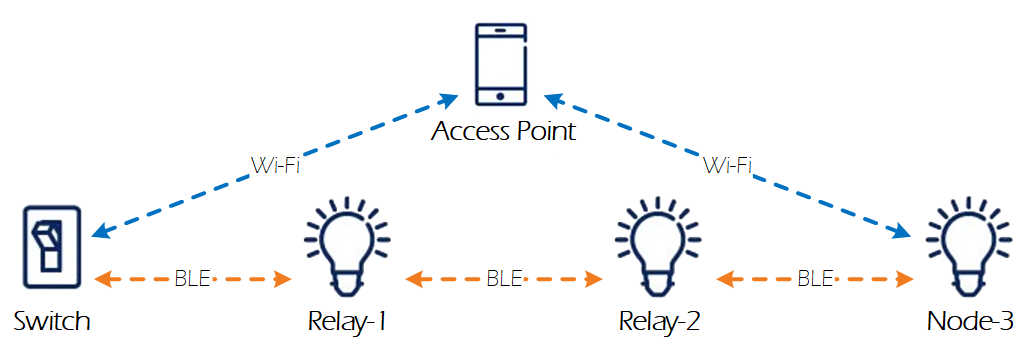
\includegraphics[width = \textwidth]{images/nodi_mesh.png}
    \caption{Ruoli rete Bluetooth mesh}
    \label{fig:ruoli_rete_mesh}
\end{figure}

\noindent Durante la fase di implementazione mi sono servito dell'ambiente di sviluppo \texttt{ESP-IDF}, poiché consente l'utilizzo di apposite librerie messa a disposizione da Espressif per la creazione di un applicativo utilizzando la tecnologia Bluetooth Mesh (la community di Espressif ha iniziato a lavorare al seguente standard solo a gennaio 2019). Al fine di evitare problematiche durante la fase implementativa in merito alle possibili modifiche giornaliere apportate dagli sviluppatori a tali librerie ho preferito focalizzare il lavoro utilizzando la versione \texttt{ESP-IDF v4.0-beta2}.\\ 

\noindent L'implementazione che consente ad un nodo di essere integrato all'interno di una rete mesh e quindi comprende l'intero processo di provisioning risulta essere identica per entrambe le tipologie di nodi (ereditata dall'esempio messo a disposizione da Espressif). Le due tipologie di ruoli, oltre a ciò, presentano un'altra caratteristica implementativa in comune, ovvero il numero di elementi di cui risultano composti. Ogni nodo è costituito da due elementi rappresentati tramite \texttt{LED} ed implementati per mezzo del modello \texttt{Generic Level Server Model}, il quale permette di comunicare l'intensità dell'illuminazione attraverso dei messaggi definiti dal \texttt{Generic Level Model}. A questi due \texttt{LED} viene aggiunto un terzo nel momento in cui viene utilizzata anche la tecnologia Wi-Fi.\\
I nodi \texttt{Relay-1}, \texttt{Relay-2} e \texttt{Node-3} presentano il medesimo codice, ad eccezion fatta per la feature \textit{relay}.\\

\noindent L'accensione di un ESP32 prevede una prima fase di inizializzazione del dispositivo a cui segue l'esecuzione dell'applicativo invocando il metodo \texttt{app\_main()}.\\
Poiché il chip ESP32 consente la memorizzazione di informazioni all'interno della memoria flash, per poter accedere a tali dati è necessario inizializzarla e per fare ciò viene utilizzata la funzione \texttt{nvs\_flash\_init()}.\\
Una volta inizializzata, si procede con l'inizializzazione degli stack da utilizzare nell'applicativo. Nel caso dell'approccio Bluetooth Mesh è necessario inizializzare per prima cosa lo stack Bluetooth Low Energy (\texttt{bluetooth\_init}) dopodiché procedere con l'inizializzazione dello standard Bluetooth Mesh (\texttt{ble\_mesh\_init}). Nel caso dell'approccio con entrambe le tecnologie, dopo avere eseguito le inizializzazioni appena descritte si procede con l'inizializzazione anche dello stack Wi-Fi.\\
Entrambi gli approcci oltre ad inizializzare gli stack relativi alle tecnologie di comunicazione da utilizzare, provvedono ad inizializzare anche dei \texttt{LED}. \\
Due \texttt{LED} utilizzati per rappresentare gli elementi di ciascun nodo e gestibili tramite lo standard Bluetooth ed un terzo \texttt{LED} gestito attraverso la tecnologia 802.11. L'impiego di tali \texttt{LED}, consente di identificare lo stato del dispositivo durante la fase di configurazione della rete Mesh ed il corretto funzionamento durante lo svolgimento della fase di test.\\
La conclusione della fase di inizializzazione viene segnalata all'utente con l'accensione di tutti i \texttt{LED} definiti per tale nodo.\\
Nel momento in cui il nodo presenta tutti i \texttt{LED} accessi allora sarà possibile procedere con il suo inserimento all'interno della rete Mesh. La definizione di tale rete avviene mediante l'applicazione \texttt{nRF Mesh}. Tale applicazione consente di individuare il dispositivo da integrare nella rete (scansionando l'ambiente circostante) e una volta individuato procedere al suo inserimento attraverso il processo di provisioning. La conclusione di tale processo viene segnalata con lo spegnimento dei \texttt{LED} associati alla tecnologia Bluetooth. Nel caso in cui l'approccio utilizzato prevede l'impiego della tecnologia Wi-Fi, al termine delle operazioni di provisioning BLE, il nodo procede automaticamente alla connessione con la rete Wi-Fi indicata (definita tramite \texttt{idf.py menuconfig}) e al termine di tale proceduta provvede a spegnere l'ultimo \texttt{LED} acceso.\\
Lo spegnimento di tutti i \texttt{LED} indica il corretto inserimento del nodo all'interno della rete e che è pronto per inviare o ricevere messaggi in base alla tecnologia supportata.\\

\noindent Durante la fase di configurazione dello stack BLE Mesh è prevista la registrazione di apposite funzioni di callback per notificare al livello applicativo il verificarsi di determinati eventi. Tali funzioni vengono innescate con la ricezione di un messaggio destinato ad uno degli elementi presenti nel nodo.\\
La ricezione e la gestione di un messaggio da parte di un elemento viene indicata all'utente cambiando lo stato del \texttt{LED} corrispondente (da \texttt{ON} ad \texttt{OFF} e viceversa). Poiché i \texttt{LED} sono l'unico strumento utilizzabile dai dispositivi per comunicare con l'utente, è stato preferito segnalare il verificarsi di questi eventi con il cambio di stato e non con variazioni graduali in base al valore contenuto nel messaggio ricevuto.

\subsection{Implementazione Client}
Il dispositivo Client, rappresentato nella figura \ref{fig:ruoli_rete_mesh} con il nome di ``\texttt{Switch}'' è quel dispositivo avente il compito di inviare i messaggi all'interno della rete mesh.\\
La natura dei messaggi è stata definita per mezzo del modello \texttt{Generic Level Model}, mentre la configurazione dell'ambiente di test (la tipologia, la frequenza d'invio, il nodo di destinazione) e quindi il comportamento del dispositivo viene comunicata per mezzo di porta seriale, avvalendosi del \texttt{USB-UART} e di uno script Python appositamente definito.\\
Poiché il seguente nodo risulta essere uno switch e quindi un interruttore generico per gestire il comportamento degli altri nodi della rete, è stato configurato utilizzando il modello \texttt{Generic Level Client Model}.
In questa sezione verrà mostrata l'implementazione del comportamento del nodo client distinguendo l'implementazione che ha permesso di definire il testbed per l'approccio Bluetooth Mesh e per l'approccio Bluetooth Mesh combinato con il Wi-Fi. Prima di descrivere i due approcci, verrà mostrato il codice appartenente al nodo Client che consente la comunicazione con il PC tramite seriale.\\

\noindent Dopo avere eseguito la configurazione delle tecnologie da utilizzare per la tipologia di approccio scelto, la prima operazione eseguita riguarda l'inizializzazione del \texttt{UART} e la definizione di un task specifico in grado di far dialogare i due dispositivi tramite porta seriale.\\

\noindent L'inizializzazione del \texttt{UART} avviene invocando la funzione \texttt{uart\_init} la quale prevede per prima cosa la configurazione del controller passando la struct \texttt{uart\_config\_t} (specificando la velocità di trasmissione, il numero di bit per ogni parola, l'utilizzo o meno di un bit di parità e la tipologia del controllo di flusso) come secondo parametro del metodo \texttt{uart\_param\_config} e come primo parametro il numero relativo al controller scelto. \\
Dopodiché si procede con la configurazione dei \texttt{PIN} ed infine si passa all'installazione del driver (\texttt{uart\_driver\_install}), andando a specificare oltre al numero del controller anche la dimensione dei buffer. L'inclusione del driver ``\texttt{driver/uart.h}'' consente di semplificare l'utilizzo di tale controller.\\

\begin{lstlisting}[language=C, caption= Configurazione e installazione driver \texttt{UART}]
void uart_init() {
    uart_config_t uart_config = {
            .baud_rate = 115200,
            .data_bits = UART_DATA_8_BITS,
            .parity = UART_PARITY_DISABLE,
            .stop_bits = UART_STOP_BITS_1,
            .flow_ctrl = UART_HW_FLOWCTRL_DISABLE
    };

    uart_param_config(UART_NUM_1, &uart_config);
    uart_set_pin(UART_NUM_1, TXD_PIN, RXD_PIN, UART_PIN_NO_CHANGE, UART_PIN_NO_CHANGE);
    uart_driver_install(UART_NUM_1, UART_BUF_SIZE * 2, 0, 0, NULL, 0);
}
\end{lstlisting}

\noindent L'utilizzo del \texttt{UART} avviene attraverso la definizione di un task (attività) specifico utilizzando il metodo \texttt{xTaskCreate}. Questo metodo richiede come parametri: il puntatore alla funzione che contiene il codice del task\footnote{I task devono essere implementati per non tornare mai}, il nome da assegnare al task (utile in fase di debugging), la dimensione dello stack di memoria (in words non in byte), i valori da passare come parametri alla funzione, la priorità con cui il task verrà eseguito e il puntatore (opzionale) per consentire la gestione del task tramite una funzione esterna. Una volta creato un task, lo scheduler di FreeRTOS lo manda in esecuzione in base alla priorità indicata.\\

\begin{lstlisting}[language=C, caption= Inizializzazione e definizione del task per utilizzare il \texttt{UART}]
void start_serial_communication(){
    uart_init();
    xTaskCreate(uart_task, "uart_task", 2048, NULL, 5, NULL);
}
\end{lstlisting}

\noindent La funzione (\texttt{uart\_task}) passata come parametro al metodo \texttt{xTaskCreate} contiene il codice che permette al nodo di essere in ascolto su una porta seriale e quindi poter ricevere un'istruzione. \\
Per acquisire i dati comunicati tramite porta seriale dal PC si utilizza l'istruzione \texttt{uart\_read\_bytes}. Una volta ricevuta la regola, il nodo procede, per prima cosa, a comprenderla (\texttt{count\_tokens}, \texttt{str\_split}) e successivamente ad attuarla adoperando la funzione \texttt{command\_received}.\\
\begin{lstlisting}[language=C, caption= acquisizione dati attraverso il \texttt{UART}]
static void uart_task(void *pvParameters) {
    uint8_t *data_uart = calloc(1, UART_BUF_SIZE);

    while (is_running_uart) {
        //Read data from the UART
        int rxBytes = uart_read_bytes(UART_NUM_1, data_uart, UART_BUF_SIZE, 100 / portTICK_RATE_MS);

        if (rxBytes > 0) {
            data_uart[rxBytes] = '\0';
            ESP_LOGI("UART", "Read %d bytes: '%s'", rxBytes, data_uart);

            char **tokens = str_split((char *) data, ',');
            command_received(tokens);

            fflush(stdout);
            uart_flush_input(UART_NUM_1);
        }
    }
    vTaskDelete(NULL);
}
\end{lstlisting}

\noindent La trasmissione di informazioni dal nodo Client al PC avviene per mezzo del dispositivo \texttt{UART} invocando l'istruzione \texttt{uart\_write\_bytes}. Tramite questa funzione si copia un array di caratteri nel buffer del driver e sarà quest'ultimo ad occuparsi, in modo autonomo, di gestire la comunicazione con il controller e l'effettivo invio dei dati. La funzione utilizzata prevede i seguenti parametri: il controller scelto, l'array di caratteri e la rispettiva dimensione. \\
La funzione riportata in seguito, \texttt{uart\_trasmitting}, prende in input un array di caratteri e dopo aver calcolato la dimensione procede a scrivere i dati nel buffer, così come descritto in precedenza.\\

\begin{lstlisting}[language=C, caption= operazione di trasmissione dati tramite lo strumento \texttt{UART}]
void uart_trasmitting(const char *event_s) {
    const int len = strlen(event_s);
    uart_write_bytes(UART_NUM_1, event_s, len);
}
\end{lstlisting}

\subsubsection{Istruzioni ed Eventi nodo Client}
\label{subsub:parametri_testbed}
Il comportamento da assumere per tale tipologia di nodo avviene attraverso una regola comunicata per mezzo di comunicazione seriale. Il nodo è in grado di acquisire tale informazione per mezzo del dispositivo \texttt{UART} (sopra descritto). L'utente, invece, può inserire tale informazione (input da tastiera) grazie ad uno script \texttt{Python} (\ref{sub:comunicazione_seriale}) in esecuzione sul PC. \\

\noindent Di seguito sono riportate le istruzioni comprensibili dal nodo client, al fine di procedere o con l'invio di un semplice messaggio utilizzando una delle tecnologie supportate oppure con l'avvio della del testbed.

\begin{itemize}
    \item la regola \texttt{``@,addr:0x0004''} (tecnologia \texttt{BLE}) impiegata per procedere all'invio di un messaggio di tipo \texttt{GET} all'indirizzo specificato.
    \item la regola \texttt{``@,addr:0x0004,level:1,type:unack''} (tecnologia \texttt{BLE}) impiegata per procedere all'invio di un messaggio di tipo \texttt{SET\_UNACK}, specificando il dato contenuto nel messaggio e l'indirizzo di destinazione.
    \item la regola \texttt{``@,addr:0x0004,level:1,type:ack''} (tecnologia \texttt{BLE}) impiegata per procedere con l'invio di un messaggio di tipo \texttt{SET}, specificando il dato contenuto nel messaggio e l'indirizzo di destinazione.
    
    \item la regola \texttt{``\#,level:1''} (tecnologia \texttt{Wi-Fi}) impiegata per procedere all'invio di un messaggio destinato a tutti i nodi appartenenti alla rete.
    
    \item la regola \texttt{``\&,n\_mex:10,addr:0x0004,delay:1000''} impiegata per attivare il testbed in base all'approccio definito a monte (\texttt{``BLE''} o \texttt{``BLE + Wi-Fi''}). La seguente regola prevede la definizione di un loop (con condizione di uscita \texttt{n\_mex}) all'interno del quale è previsto l'invio di un messaggio ad un nodo specifico (\texttt{addr}). Ogni iterazione avviene con una cadenza definita dal valore indicato da \texttt{delay}.

\end{itemize}
\noindent Le prime quattro regole servono esclusivamente a verificare che tutto sia stato configurato correttamente, infatti consentono di inviare un semplice messaggio contenente le informazioni indicate dal campo \texttt{level}, mentre la quinta regola consente di configurare i parametri necessari per il test ed avviare la simulazione. L'indirizzo di destinazione, assegnato durante la fase di provisioning, identificata in modo univoco l'elemento presente su uno dei nodi della rete a cui risulta essere destinato il messaggio (espresso sia con \texttt{0x0004} o con \texttt{4}).\\

\noindent L'impiego del \texttt{UART} in fase trasmissiva consente di comunicare uno dei seguenti eventi (invio, ricezione, errore del messaggio) verificati sul nodo, i quali consentono al termine del testbed di creare un file di log su cui si basano le successive analisi. L'array di caratteri comunicato può essere descritto semplicemente come una stringa costituita dai seguenti tre campi: \texttt{event} (indica il tipo di evento accaduto), \texttt{level} (corrisponde all'identificativo del messaggio) e \texttt{TTL} (indica il valore \textit{time-to-live} contenuto nel messaggio (in questo contesto compreso tra 0 e 3).\\
La costruzione della suddetta stringa avviene comunicando i tre array di caratteri alla seguente funzione, \texttt{event\_reporting}. Una volta concatenati i dati ricevuti procede con la comunicazione al PC attraverso il metodo descritto in precedenza, ovvero \texttt{uart\_trasmitting}. Tale funzione prevede un quarto parametro che consente di mostrare sulla console (accessibile con il comando \texttt{idf.py -p PORT monitor}) l'evento verificatosi utilizzando apposite \texttt{macro} messe a disposizione dalla libreria \texttt{esp\_log.h}.\\

\begin{lstlisting}[language=C, caption= costruzione stringa da inviare al PC tramite \texttt{uart\_trasmitting}]
void event_reporting(char *status, char *level, char *ttl, uint8_t show_log) {
    char *str3 = malloc(1 + 2 + strlen(status) + strlen(level) + strlen(status));// 1 end char; 2 for comma

    strcpy(str3, status);
    strcat(str3, ",");
    strcat(str3, level);
    strcat(str3, ",");
    strcat(str3, ttl);

    uart_trasmitting(str3);
    free(str3);

    if (show_log == 1) {
        if (strcmp(status, "I") == 0 || strcmp(status, "S") == 0) {
            ESP_LOGI("PC", "[status: %s, level: %s ttl: %s]", status, level, ttl);
        } else if (strcmp(status, "R") == 0 || strcmp(status, "O") == 0) {
            ESP_LOGW("PC", "[status: %s, level: %s ttl: %s]", status, level, ttl);
        } else {
            ESP_LOGE("PC", "[status: %s, level: %s ttl: %s]", status, level, ttl);
        }
    }
}
\end{lstlisting}

\noindent Di seguito sono descritte le stringhe inviabili dal client verso il PC in base alla tipologia di evento sollevato (invio, ricezione ed errore), ma anche in base alla tecnologia che lo ha innescato. \\
La lettera iniziale identifica l'evento e la tecnologia, il secondo valore coincide con l'identificativo del messaggio ed il terzo con il time-to-live.
\begin{itemize}
    \item \textit{\texttt{invio}}:
    \begin{itemize}
        \item \texttt{``S,1,3''} indica l'invio di un messaggio con identificativo pari ad \texttt{1} attraverso la tecnologia \texttt{Bluetooth Mesh}.
        
        \item \texttt{``I,1,3''} indica l'invio di un messaggio con l'identificativo \texttt{1} attraverso la tecnologia \texttt{Wi-Fi}.
    \end{itemize}

    \item \textit{\texttt{ricezione}}:
    \begin{itemize}
        \item \texttt{``R,1,3''} indica la ricezione di un messaggio con \texttt{TTL} pari a 3 e con identificativo pari ad \texttt{1}, tramite la tecnologia \texttt{Bluetooth Mesh}.
        
        \item \texttt{``O,1,3''} indica la ricezione di un messaggio con \texttt{TTL} pari a 3 e con identificativo pari ad \texttt{1}, tramite la tecnologia \texttt{Wi-Fi}.
    \end{itemize}
    
    \item \textit{\texttt{errore}}:
    \begin{itemize}
        \item \texttt{``E,1,0''} indica la presenza di un errore in fase d'invio e quindi il messaggio con identificativo \texttt{1} non viene inviato. (\texttt{Bluetooth Mesh})
        
        \item \texttt{``W,1,0''} indica la presenza di un errore in fase d'invio del messaggio con identificativo \texttt{1}. (\texttt{Wi-Fi})
    \end{itemize}
\end{itemize}

\subsubsection{Approccio BLE Mesh}
\label{subsub:BLE}
Il testbed relativo al seguente approccio prevede esclusivamente l'invio di messaggi, adottando la tecnologia Bluetooth Mesh, in base ai parametri definiti dalla regola ricevuta. Tale regola viene memorizzata in una \texttt{struct} per agevolare il suo utilizzo all'interno del codice.\\
Prima di avviare il test vengono inizializzate le seguenti variabili: \texttt{level} (usata per identificare un messaggio e definire lo stato da assumere per l'elemento destinatario del messaggio), \texttt{xDelay} (usata per indicare il delay tra due messaggi consecutivi). Dopo aver definito la \texttt{struct} e inizializzato le variabili viene definito un loop all'interno del quale vengono inviati i messaggi nella rete. Tale ciclo è definito in modo tale da avere sempre la stessa durata del test, indipendentemente dalla frequenza d'invio utilizzata.\\

% https://www.freertos.org/vtaskdelayuntil.html
\noindent La frequenza d'invio viene scandita utilizzando il metodo \texttt{vTaskDelayUntil} di \texttt{FreeRTOS}. La scelta è ricaduta su tale funzione poiché essa assicura, per un task periodico, una frequenza d'esecuzione constante. Ovvero, prevede lo sblocco del task, e quindi l'invio del messaggio, in un momento ben preciso (assoluto). 
Contrariamente, l'altra funzione messa a disposizione da \texttt{FreeRTOS} (\texttt{vTaskDelay}), determinata l'istante di sblocco dell'attività a partire dal momento in cui risulta invocata (relativo). Così facendo non permette di avere una frequenza d'esecuzione fissa poiché influenzata dal tempo impiegato per l'invio del messaggio e per la comunicazione dell'evento al PC.\\

\noindent Indipendentemente dalla funzione utilizzata, \texttt{FreeRTOS} mette in pausa il task per un numero di ticks specificati come parametro. La constante \texttt{portTICK\_PERIOD\_MS} definisce la durata, in millisecondi, di un tick. Il numero di ticks equivalenti al valore di delay comunicato, espresso in millisecondi, si ottiene dividendo tale valore per la costante \texttt{portTICK\_PERIOD\_MS}.\\

\noindent L'operazione di \textit{invio} è caratterizzata dall'invio effettivo del messaggio Bluetooth Mesh, \texttt{send\_message\_BLE}, e dalla segnalazione di tale evento al PC avvalendosi della funzione \texttt{event\_reporting}. La funzione \texttt{send\_message\_BLE} richiede rispettivamente: l'indirizzo del destinatario (\texttt{rule.addr}), la tipologia di messaggio inviato (\texttt{LEVEL\_SET\_UNACK}), l'identificativo del messaggio nonché il valore da comunicare al client (\texttt{level}) e l'impiego o non impiego del metodo di conferma implementato dallo standard Bluetooth Mesh (\texttt{rule.ack}). Come indicato nel capitolo \nameref{ch:progettazione}, è stato definito un metodo di conferma personalizzato (descritto nella sottosezione \nameref{sub:implementazione server}) poiché quello implementato dallo standard non consente di valutare il comportamento della rete con un carico di lavoro elevato.\\

\begin{lstlisting}[language=C, caption= evento di invio di un messaggio Bluetooth Mesh]
void execute_rule() {
    int16_t level = 1;
    char level_c[7];

    const TickType_t xDelay = rule.delay / portTICK_PERIOD_MS;
    TickType_t xLastWakeTime = xTaskGetTickCount();

    for (int i = 0; i < rule.n_mex; ++i) {
        vTaskDelayUntil(&xLastWakeTime, xDelay);
        send_message_BLE(rule.addr, ESP_BLE_MESH_MODEL_OP_GEN_LEVEL_SET_UNACK, level);
        
        sprintf(level_c, "%d", level);
        event_reporting("S", (char *) level_c, "3");
        
        level += 1;
    }
}
\end{lstlisting}

\noindent L'operazione di \textit{ricezione} di un messaggio viene innescata attraverso gli eventi definiti dallo stack Bluetooth Mesh. Poiché la gestione del messaggio di risposta sul nodo server è stata personalizzata (per i motivi descritti nel capitolo \nameref{ch:progettazione}), l'evento che sancisce la conferma di ricezione del messaggio corrisponde a \texttt{ESP\_BLE\_MESH\_GENERIC\_CLIENT\_PUBLISH\_EVT}. Al verificarsi di tale evento, si procede innanzitutto definendo due array di caratteri per convertire in stringa i parametri \texttt{TTL} e \texttt{level} contenuti nel messaggio ricevuto, e poi con la comunicazione dell'evento al PC.\\

\begin{lstlisting}[language=C, caption= evento di ricezione e errore in fase d'invio]
switch (event) {
    ...
    case ESP_BLE_MESH_GENERIC_CLIENT_PUBLISH_EVT: {
        char level[7];
        char ttl[4];
        sprintf(level, "%d", param->status_cb.level_status.present_level);
        sprintf(ttl, "%d", param->params->ctx.recv_ttl);
        
        event_reporting("R", level, ttl);
        break;
    }
    ...
    case ESP_BLE_MESH_GENERIC_CLIENT_SET_STATE_EVT: {
        ...
        if (param->params->opcode == ESP_BLE_MESH_MODEL_OP_GEN_LEVEL_SET_UNACK) {
            char info_level[7];
            sprintf(info_level, "%d", my_info_level);
            event_reporting("E", info_level, "0");
        }
        ...
        break;
    }
    ...
}
\end{lstlisting}

\noindent L'evento di \textit{errore} è individuato con il verificarsi dell'evento \texttt{ESP\_BLE\_MESH\_GENERIC} \texttt{\_CLIENT\_SET\_STATE\_EVT}.\\ All'interno di tale evento è stato necessario analizzare l'\texttt{opcode} del messaggio per determinare se si tratta effettivamente di un'errore. L'errore riscontrato si verifica nel momento in cui il buffer di trasmissione del livello di rete risulta essere pieno.\\
Con l'approccio Bluetooth Mesh, al verificarsi di tale errore viene solo eseguita una comunicazione al PC attraverso l'istruzione \texttt{event\_reporting}, ma non si attua nessuna strategia per ripetere l'operazione non appena il buffer risulta nuovamente libero.

\subsubsection{Approccio BLE Mesh più Wi-Fi}
\label{subsub:BLE_WiFi}
Il seguente approccio è stato definito dopo aver analizzato i risultati del primo in cui si è evidenziato un elevato numero di errori e quindi il mancato invio dei pacchetti (ai fini statistici conteggiati come pacchetti persi). A tal proposito è stata introdotta la tecnologia 802.11 come supporto per limitare le perdite di pacchetto.\\
In merito all'uso della tecnologia Bluetooth Mesh resta tutto invariato ad eccezione del fatto che è stato necessario introdurre un buffer per gestire i pacchetti persi in tempo reale.\\

\noindent In questo caso, dopo aver inizializzato ed avviato il task per consentire la comunicazione tra dispositivo e PC, è stata definita una socket al fine di instaurare una comunicazione basata sulla tecnologia 802.11 (pila TCP/IP) all’interno della rete. Gli elementi necessari per il funzionamento di una comunicazione tramite socket sono: l'indirizzo IP e il numero di porta. Tali elementi consento di distinguere in maniera univoca le singole richieste all'interno della rete.\\
La tipologia di socket utilizzata in questo contesto è \texttt{Datagram Socket} il che consente una comunicazione basata sul protocollo UDP. Vale a dire che l'invio dei messaggi avviene mediante il trasferimento di datagrammi senza dover garantire il corretto ordine d'arrivo, la correttezza dell'informazione e soprattutto senza che client e server debbano instaurare una vera e propria connessione, ma il client comunica direttamente con il server, quando vuole.\\

\noindent La definizione della socket avviene tramite il metodo \texttt{socket} messo a disposizione dalla libreria \texttt{lwip/sockets.h} in cui bisogna specificare il dominio (\texttt{AF\_INET}), il tipo (\texttt{SOCK\_DGRAM}) e il protocollo (\texttt{IPPROTO\_IP}). In cui \texttt{AFF\_INET} specifica l'impiego di un indirizzo \texttt{ip} di 32 bit e un numero di porta a 16 bit, \texttt{SOCK\_DGRAM} indica la definizione di una \texttt{Datagram Socket} e \texttt{IPPROTO\_IP} indica l'impiego del protocollo \texttt{ip} per l'invio e la ricezione dei messaggi.\\

\begin{lstlisting}[language=C, caption= creazione della socket]
void create_socket() {
    addr_family = AF_INET;
    ip_protocol = IPPROTO_IP;

    while (1) {
        sock = socket(addr_family, SOCK_DGRAM, ip_protocol);
        if (sock < 0) {
            ESP_LOGE(TAG, "Unable to create socket: errno %d", errno);
        }
        ESP_LOGI(TAG, "Socket created, port: %d", PORT);
        break;
    }
    is_running_wifi = true;
}
\end{lstlisting}

\noindent Una volta definita la socket viene avviato il task (\texttt{udp\_client\_receive}) che consente al nodo di poter ricevere messaggi a lui destinati attraverso la tecnologia 802.11, sempre tramite l'istruzione \texttt{xTaskCreate}. In tal caso, alla ricezione di un messaggio il nodo provvede a comunicarlo tempestivamente al PC tramite il metodo \texttt{uart\_trasmitting} in cui viene passato come parametro l'array di caratteri identificante tale evento (le tipologie di stringhe correlate agli eventi comunicati dal nodo client sono descritte nella sottosezione \nameref{subsub:parametri_testbed}). La definizione del seguente task in questo momento consente non solo di ricevere messaggi di tipo \texttt{ip} durante il testbed ma anche quando si impiegano le altre regole precedentemente descritte.\\

\noindent La struttura (denominata buffer) che consente di memorizzare gli identificativi dei messaggi e quindi la gestione dei messaggi in tempo reale risulta implementata mediante una struttura dati di tipo \texttt{coda}. Le operazioni previste per la seguente struttura dati riguardano l'inserimento in coda dell'identificativo del messaggio (\texttt{enQueue}), la due procedure di rimozione, la prima consente di rimuovere un messaggio dalla testa della coda (\texttt{deQueue}), mentre la seconda prevede per primo la ricerca dell'identificativo all'interno della coda ed in seguito, in caso di esito positivo, la rispettiva rimozione (\texttt{remove\_key}). L'operazione \texttt{deQueue} è l'unica che prevede un unico parametro, ovvero la coda, mentre le altre due prevede anche l'identificativo da inserire o rimuovere, a seconda dei casi. Queste due operazioni sono invocate mediante la funzione \texttt{queue\_operation} in base ai parametri ricevuti in input. I parametri necessari riguardano il tipo di operazione (\texttt{`a'} o \texttt{`d'}), la tecnologia del messaggio (\texttt{`b'} o \texttt{`w'}) e l'identificativo. Oltre a gestire le operazioni con la coda, solo ed esclusivamente con l'evento di ricezione di un messaggio Bluetooth prevede ad invocare il metodo \texttt{update\_delay\_buffer} per aggiornare il valore relativo al delay dinamico.\\

\noindent L'istruzione di \textit{invio} (eseguita sempre all'interno di un loop, come indicato nell'approccio Bluetooth Mesh) prevede, dopo le operazioni di invio del messaggio (\texttt{send\_message\_BLE}) e la comunicazione di tale evento (\texttt{event\_reporting}), l'inserimento dell'identificativo all'interno del buffer (attraverso l'operazione \texttt{enQueue} invocata all'interno della funzione \texttt{queue\_operation} con i parametri impostati come nel blocco di codice che segue). 

\begin{lstlisting}[language=C, caption= evento d'invio con rispettiva segnalazione e utilizzo della coda]
void send_message_BLE(uint16_t addr, uint32_t opcode, int16_t level) {
    esp_ble_mesh_generic_client_set_state_t set = {{0}};
    esp_ble_mesh_client_common_param_t common = {0};
    esp_err_t err;

    common.opcode = opcode;
    common.model = bleMeshClient.model;
    common.ctx.net_idx = node_net_idx;
    common.ctx.app_idx = node_app_idx;
    common.ctx.addr = addr;
    common.ctx.send_ttl = 3;
    common.ctx.send_rel = false;
    common.msg_timeout = 0;
    common.msg_role = ROLE_NODE;

    set.level_set.op_en = false;
    set.level_set.level = level;
    set.level_set.tid = msg_tid++;
    my_info_level = level;

    err = esp_ble_mesh_generic_client_set_state(&common, &set);
    char level_c[7];
    sprintf(level_c, "%d", level);    
    if (err) {
        event_reporting("W", level_c, "0", 1);
    } else {
        event_reporting("S", level_c, "3", 1);
    }
    queue_operation('a', 'b', level);
}
\end{lstlisting}

\noindent L'operazione di \textit{ricezione} di un messaggio tramite la tecnologia Bluetooth Mesh prevede la comunicazione dell'evento, così come avviene con l'approccio descritto in precedenza, ma a tale operazione segue la rimozione dal buffer dell'identificativo corrispondente al messaggio ricevuto (\texttt{remove\_key}).

\paragraph{Algoritmo dinamico} 
L'algoritmo dinamico, che consente l'impiego della tecnologia Wi-Fi all'interno del testbed, prevede due fasi: durante la prima fase resta in uno stato dormiente, denominato transiente iniziale, mentre durante la seconda provvede, all'interno di un loop, utilizzando utilizzando la medesima frequenza specificata per il seguente testbed, l'invio di messaggi utilizzando l'identificativo estratto dalla coda mediante la funzione \texttt{deQueue}.\\
La prima fase ha una durata di $40 s$ a partire dall'invio del primo messaggio del testbed e tale tempo viene verificato in termini di messaggi inviati. Ad esempio se la regola impostata prevede l'invio di un messaggio ogni $50 ms$, allora vorrà dire che la condizione dei $40 s$ di attesa scadrà a seguito dell'invio del ottocentesimo pacchetto ($40 s\div 50 ms = 800$). In tale circostanza, $800$ coincide proprio con il valore contenuto della variabile \texttt{delay\_buff\_init}.\\
Verificata tale condizione si passa quindi alla seconda fase, la quale garantisce la possibilità di inviare un messaggio (\texttt{send\_mex\_wifi}) solo se la differenza tra l'identificativo contenuto nel messaggio corrente (\texttt{level\_sent}) e l'identificativo presente in testa alla coda (\texttt{front\_value}) risulta maggiore del delay dinamico (\texttt{delay\_buffer}). Inizialmente il valore dinamico è impostato a $40 s$, adottando sempre il meccanismo di conversione sopra descritto. Solo se risulta soddisfatta la condizione appena descritta è possibile procedere con l'operazione di invio adottando la tecnologia 802.11. La quale prevede: l'estrazione dell'elemento in testa alla coda, l'invio del messaggio con l'identificativo estratto e la segnalazione di tale evento al PC.\\

\begin{lstlisting}[language=C, caption= algoritmo dinamico e invio messaggio tramite Wi-Fi]
void get_key_and_send_mex() {
    int front_value = get_front_key(q_ble);
    if (front_value > 0) {
        if ((level_sent - front_value) > (int) delay_buffer) {
            int value = deQueue(q_ble);
            send_mex_wifi(value);
        }
    }
}

void send_mex_wifi(int16_t value) {
    sprintf(payload, "%d", value);
    int err = sendto(sock, payload, strlen(payload), 0, (struct sockaddr *) &dest_addr, sizeof(dest_addr));
    if (err < 0) {
        ESP_LOGE(TAG, "Error occurred during sending: errno %d", errno);
        event_reporting("W", payload, "0", 1);
    } else {
        event_reporting("I", payload, "0", 1);
        queue_operation('a', 'w', value);
    }
}

static void udp_client_sent(void *pvParameters) {
    TickType_t xLastWakeTime = xTaskGetTickCount();
    const TickType_t xDelay = rule.delay_s / portTICK_PERIOD_MS;

    while (is_running_rule) {
        vTaskDelayUntil(&xLastWakeTime, xDelay);
        if (level_sent >= delay_buff_init) {
            get_key_and_send_mex();
            if (!change_delay) {
                change_delay = true;
            }
        }
    }
    vTaskDelete(NULL);
}
\end{lstlisting}

\noindent Il cuore dell'algoritmo dinamico è rappresentato dal codice seguente il quale consente di aggiornare il valore della soglia (\texttt{threshold}) in funzione delle condizioni della rete. La condizione posta all'inizio (\texttt{if(change\_delay)}) consente di aggiornare tale valore solo a seguito del transiente iniziale. Il valore di soglia viene aggiornato con le seguenti formule:

$$ delay\_estimation = threshold_{t_0} + \alpha \times (R-threshold_{t_0}) $$
$$ threshold_{t_1} = \beta \times  delay\_estimation $$

\noindent La formula \texttt{delay\_estimation} consente di calcolare il nuovo \textit{delay} al fine di considerare un pacchetto come perso in base allo stato della rete. In tale formula: 
\begin{itemize}
    \item $threshold_{t_0}$ esprime il valore attuale della soglia.
    \item $\alpha$ indica il \textit{learning rate}, ovvero il tasso con cui le nuove informazioni acquisite hanno incidenza sulle quelle vecchie e rappresenta la velocità con cui il modello aggiorna la propria conoscenza in merito allo stato della rete. Un fattore pari a \texttt{0} fa sì che l'agente non impara nulla (sfrutta solo la conoscenza pregressa) ed un fattore pari a \texttt{1} fa sì che l'agente considera solo le informazioni recenti, tralasciando la base di conoscenza pregressa. Eseguendo diverse prove è stato possibile definire il valore $\alpha$ pari a $0.2$. 
    \item $R$ indica lo stato attuale della rete (valore ottenuto dalla differenza tra l'identificativo contenuto nell'ultimo messaggio inviato, \texttt{level\_sent}, e l'identificativo contenuto nel pacchetto ricevuto, \texttt{key}).
\end{itemize}
\noindent La formula \texttt{$threshold_{t_1}$} consente di stimare il nuovo valore di soglia affinché un pacchetto venga considerato perso in base alla situazione corrente della rete (in termini di latenza).\\
Per essere più confidenti nell'aggiornare la soglia e quindi evitare scelte troppo affrettate, tale valore (\texttt{delay\_estimation}) viene moltiplicato per una costante, \texttt{$\beta$}. L'introduzione di tale constante consente quindi un'alterazione piuttosto dolce del valore di soglia in modo da poter andare a considerare anche i pacchetti con una latenza leggermente maggiore della media come ``correttamente ricevuti'' e non giudicarli frettolosamente come ``persi''. Lavorando in questo modo, concedendo una soglia leggermente più ampia della latenza attuale della rete, il nodo tende ad evitare l'invio di informazioni ridondanti e così un maggior dispendio di energie necessarie per l'invio di un pacchetto impiegando la tecnologia \texttt{Wi-Fi}. A seguito di diversi test il valore $\beta$ è stato definito pari a \texttt{1.1}.\\

\noindent Il nuovo valore di soglia, che verrà calcolato a seguito della ricezione di un messaggio \texttt{BLE}, risulterà essere compreso in un intervallo di $[1s, 40s]$ espresso in termine di messaggi inviati (rispettivamente indicato dalle variabili \texttt{threshold\_min} e \texttt{threshold\_max}).\\

\begin{lstlisting}[language=C, caption= aggiornamento del valore di soglia]
void update_delay_threshold(int key) {
    if (change_delay) {
        // delay_ = t_0 + alpha*(R - t_0)
        // t_1 = 1.1*(delay_)
        // alpha = 0.2 --- 1-alpha = 0.8
        int status = level_sent - key;
        double threshold_1 = 1.1 * ((0.2 * status) + (0.8 * threshold));

        int threshold_0 = (int) threshold;
        if (threshold_1 >= threshold_min && threshold_1 <= threshold_max) {
            threshold = threshold_1; // a <= threshold <= b
        } else if (threshold_1 > threshold_max) {
            threshold = threshold_max; // threshold > b
        } else {
            threshold = threshold_min; // threshold < a
        }
    }
}
\end{lstlisting}

\noindent In merito all'operazione di \textit{ricezione} è stato definito un task (\texttt{udp\_client\_receive}) dotato di un loop in cui il nodo risulta sempre in attesa di ricevere un messaggio. Alla sua ricezione si procede semplicemente con la segnalazione dell'evento (utilizzando l'identificativo del messaggio) al PC. Non vengono effettuati controlli sul mittente perché si ha l'assoluta certezza che oltre al nodo Client non c'è nessun altro dopo in grado di inviare messaggi senza prima essere stato contattato dal Client.\\

\begin{lstlisting}[language=C, caption= metodo di ricezione Wi-Fi]
static void udp_client_receive(void *pvParameters) {
    struct sockaddr_in source_addr;
    socklen_t socklen = sizeof(source_addr);

    while (is_running_wifi) {
        int len = recvfrom(sock, rx_buffer, sizeof(rx_buffer) - 1, 0, (struct sockaddr *) &source_addr, &socklen);

        if (len < 0) { 
            // Error occurred during receiving
            ESP_LOGE(TAG, "recvfrom failed: errno %d", errno);
        } else {
            rx_buffer[len] = 0; // Null-terminate
            event_reporting("O", rx_buffer, "*", 1);
        }
    }
    vTaskDelete(NULL);
}
\end{lstlisting}

\subsection{Implementazione Server}
\label{sub:implementazione server}
Come indicato nell'introduzione del seguente capitolo, i due dispositivi \texttt{Relay} e il dispositivo \texttt{Node-3} assumono il ruolo di Server all'interno della rete Bluetooth Mesh poiché consentono ai nodi di tipo Client  di accedere e gestire gli elementi di cui risultano composti. 
I nodi indicati \texttt{Relay-1} e \texttt{Relay-2} supportano la funzione \textit{relay}, vale a dire che nel momento in cui ricevono un messaggio non destinato a loro, provvedono ad inoltrarlo ai propri vicini. Tale tecnica ha permesso le realizzazione di una rete mesh su un ambiente piuttosto ampio. L'utilizzo di tale feature deve essere abilitata in fase di configurazione del nodo (dal menu ottenibili dal comando \texttt{idf.py menuconfig} e poi attivata in fase di inizializzazione del nodo, attraverso la costante \texttt{ESP\_BLE\_MESH\_RELAY\_ENABLED}.\\ 

\begin{lstlisting}[language=C, caption= attivazione feature \textit{relay}]
static esp_ble_mesh_cfg_srv_t config_server = {
        .relay = ESP_BLE_MESH_RELAY_ENABLED,
        .beacon = ESP_BLE_MESH_BEACON_ENABLED,
        .friend_state = ESP_BLE_MESH_FRIEND_NOT_SUPPORTED,
        .gatt_proxy = ESP_BLE_MESH_GATT_PROXY_NOT_SUPPORTED,
        .default_ttl = 3,
        .net_transmit = ESP_BLE_MESH_TRANSMIT(2, 20),
        .relay_retransmit = ESP_BLE_MESH_TRANSMIT(2, 20),
};
\end{lstlisting}

\noindent Il dispositivo \texttt{Node-3} non prevede l'utilizzo di tale funzionalità, quindi viene disabilitata attraverso la costante \texttt{ESP\_BLE\_MESH\_RELAY\_DISABLED}.\\
Di seguito verrà mostrata l'implementazione del comportamento di un nodo Server alla ricezione di un messaggio distinguendolo in base alla tecnologia utilizzata.\\

\subsubsection{Bluetooth Mesh}
La ricezione di un messaggio Bluetooth su un nodo viene individuata attraverso un evento gestito dalla funzione di callback \texttt{example\_ble\_mesh\_generic\_server\_cb}. Il verificarsi di tale evento consente la gestione del messaggio ricevuto a livello applicativo. Una volta individuata la tipologia di messaggio ricevuto (\texttt{GET}, \texttt{SET} e \texttt{SET\_UNACK}) si procede con l'operazione corrispondente.\\
Per il messaggio di tipo \texttt{GET} è prevista una risposta contenente lo status del relativo elemento.
Per il messaggio di tipo \texttt{SET} è prevista l'attuazione del comando ricevuto e l'invio di una conferma di ricezione al mittente.
Per il messaggio di tipo \texttt{SET\_UNACK} normalmente è prevista solo l'attuazione del comando ricevuto, però ai fine del seguente lavoro è stato necessario apportare delle modifiche affinché potessimo testare la rete con un carico di lavoro elevato e allo stesso tempo tener traccia dei messaggi giunti a destinazione (conferma di ricezione). I motivi per cui non è stato possibile l'impiego dei messaggi di tipo \texttt{SET} è descritto nel capitolo di \nameref{ch:progettazione}.\\

\noindent Il meccanismo implementato prevede l'utilizzo di messaggi di tipo \texttt{SET\_UNACK}. Alla ricezione di tale tipologia di messaggio viene innescato l'evento \texttt{ESP\_BLE\_MESH\_} \texttt{GENERIC\_SERVER\_RECV\_SET\_MSG\_EVT} in grado di gestire entrambe le tipologie di messaggi di tipo \texttt{SET}. Per distinguerle e lavorare solo con la tipologia di interesse è necessario accedere al contesto del messaggio. Da tali informazioni otteniamo sia il codice operativo (\texttt{recv\_op}) sia ulteriori informazioni in merito alla natura del messaggio. Dopo aver verificato il codice operativo si procede ad estrarre i dati contenuti nel messaggio in base al modello scelto (\texttt{Generic Level Set}). Ottenuto l'identificativo del messaggio (\texttt{level}) è possibile generare un messaggio di risposta il che garantirà al mittente la conferma di ricezione del messaggio avente tale identificativo. Il messaggio di risposta risulta essere di tipo \texttt{STATUS} e conterrà lo stesso identificativo del messaggio ricevuto dal nodo Server. Una volta immesso nella rete tale messaggio si procede ad attuare il cambiamento di stato corrispondente all'elemento destinatario di tale messaggio. Il cambiamento di stato in questa circostanza prevede l'accensione o lo spegnimento del \texttt{LED}, in base allo stato precedente. Con questo metodo anche l'utente è in grado di percepire lo svolgimento di tale operazione da parte del nodo e quindi assicurarsi che il test sta procedendo correttamente.\\

\begin{lstlisting}[language=C, caption= gestione messaggi di tipo \texttt{SET\_UNACK}]
switch (ctx->recv_op) {
        case ESP_BLE_MESH_MODEL_OP_GEN_LEVEL_SET:
        ...
        case ESP_BLE_MESH_MODEL_OP_GEN_LEVEL_SET_UNACK:
            srv->state.level = set->level;
            ctx->send_ttl = 3;
            
            esp_ble_mesh_server_model_send_msg(model, ctx, ESP_BLE_MESH_MODEL_OP_GEN_LEVEL_STATUS, sizeof(srv->state.level), (uint8_t *) &srv->state.level);

            change_led_state(model, ctx);
            break;
        ...
    }
\end{lstlisting}

\subsubsection{Wi-Fi}
Per quanto riguarda l'impiego della tecnologia Wi-Fi, come accade per il nodo Client, bisogna innanzitutto definire una socket e dopodiché viene definito un task (\texttt{udp\_server\_task}) costituito da un loop tramite il quale il nodo risulta essere sempre in attesa di dati. In tale circostanza, a differenza del nodo Client, la ricezione di un pacchetto non comporta la comunicazione dell'evento al PC, poiché tale tipologia di nodo non è collegato ad esso. La ricezione di un pacchetto prevede l'estrazione dell'identificativo in esso contenuto, la creazione e il rinvio di un messaggio di risposta ed infine il cambiamento di stato del \texttt{LED} relativo alla tecnologia Wi-Fi.

\begin{lstlisting}[language=C, caption= ricezione messaggio Wi-Fi su un nodo Server]
static void udp_server_task(void *pvParameters) {
    struct sockaddr_in source_addr; // IPv4
    socklen_t socklen = sizeof(source_addr);


    ESP_LOGI(TAG, "Waiting for data");
    while (is_running_wifi) {
        int len = recvfrom(sock, rx_buffer, sizeof(rx_buffer) - 1, 0, (struct sockaddr *) &source_addr, &socklen);

        if (len < 0) {
            ESP_LOGE(TAG, "recvfrom failed: errno %d", errno);
        } else {
            // Get the sender's ip address as string
            inet_ntoa_r(((struct sockaddr_in *) &source_addr)->sin_addr.s_addr, addr_str, sizeof(addr_str) - 1);

            rx_buffer[len] = 0; // Null-terminate whatever we received and treat like a string...
            ESP_LOGW(TAG, "Received %d bytes from %s: [%s]", len, addr_str, rx_buffer);

            send_mex_wifi(len, source_addr);
            board_led_operation_wifi(LED_WIFI, status_led_wifi);
            status_led_wifi = !status_led_wifi;
        }
    }
    vTaskDelete(NULL);
}
\end{lstlisting}

\subsection{Comunicazione Seriale}
\label{sub:comunicazione_seriale}
Come indicato in precedenza la comunicazione seriale tra il PC e il nodo Client è garantita attraverso uno script \texttt{Python} in esecuzione sul PC. Oltre a consentire la comunicazione tra i due dispositivi tramite seriale (avvalendosi della libreria \texttt{serial}) esso consente di verificare se la regola immessa dall'utente possa essere interpretata correttamente dal nodo al fine di evitare eventuali crash. Oltre a ciò prevede la creazione di un file di log contenente tutti gli eventi generati dal nodo e comunicati rispettando un formato prestabilito.\\

\noindent Lo script prevede l'esecuzione dei seguenti due task in parallelo, il task \texttt{write\_on\_} \texttt{serial} per la definizione della regola da comunicare al nodo e il task \texttt{read\_from\_} \texttt{serial} per essere sempre in ascolto della seriale in modo da poter ricevere i dati comunicati dall'altro dispositivo.\\

\begin{lstlisting}[language=Python, caption= scrittura su porta seriale e validazione input]
def write_on_serial():
    global save_data

    while True:
        reading()
        try:
            command = input("Enter the command to be sent to the esp32: \n")

            if re.match(regular_expresion_command, command) or re.match(regular_expresion_set_get, command) or re.match(regular_expresion_rule, command) or re.match(regular_expresion_wifi, command):
                if command == 'q' or command == 'e':
                    if command == 'q':
                        save_data = True
                        print("Waiting for Save")
                    event.set()
                    break
                elif command == 'p':
                    my.print_data_as_json(data)
                else:
                    esp32.write(command.encode())
                    add_command_to_dictionary(command)
            else:
                print('\x1b[6;30;41m' + "Wrong command" + '\x1b[0m')

        except KeyboardInterrupt:
            event.set()
            break
\end{lstlisting}

\noindent Prima di procedere con la comunicazione all'esp32, l'input immesso dall'utente viene validato tramite l'impiego di espressione regolari affinché rispetti una delle cinque regole comprensibili dal nodo. Le regole sono definite in modo da consentire all'utente di adattarle alla circostanza della rete. Se l'esito di tale validazione risulterà positivo allora si procederà con la comunicazione altrimenti verrà chiesto all'utente di inserire nuovamente la regola. Oltre alle regole, di seguito descritte, sono stati definiti ulteriori comandi per eseguire operazioni in locale come la stampa a video degli eventi comunicati dal Client (con il comando \texttt{`p'}) e la terminazione dello script (il comando \texttt{`q'} consente di terminare e salvare il file di log e il comando \texttt{`w'} per chiudere senza salvare). Di seguito sono riportate le tre espressioni regolari utilizzate per validare l'input inserito.

\begin{itemize}
    \item ``\verb/^@,addr:(((0x){1}[a-fA-F-0-9]{4})|([0-9]{1,2}))(,level:[0-9]{1,/  \verb/5}(,ack:[0|1]){0,1}){0,1}$/'' consente di validare le regole relative alla tecnologia Bluetooth Mesh.
    
    \item ``\verb/^#,level:[0-9]{1,5}$/'' consente di validare la regola relativa alla tecnologia Wi-Fi.
    
    \item ``\verb/^&,n_mex:[0-9]{1,5},addr:([0-9]{1,2}|0x[a-fA-F-0-9]{4}),delay:/\\  \verb/[0-9]{1,6}$/'' consente di validare la regola per avviare la procedura di testbed.
\end{itemize}

\noindent L'altro task in esecuzione all'interno del script consente di ricevere tutti gli eventi verificatosi sull'esp32 e creare il file di log. Alla ricezione di un'informazione tramite porta seriale viene immediatamente calcolato il timestamp dell'operazione e si procedere ad aggiungere i dati all'interno di un dictionary. Al termine del testbed, l'utente può scegliere se il dizionario creato debba essere salvato prima chiudere lo script oppure può essere rimosso. 

\begin{lstlisting}[language=Python, caption= lettura tramite porta seriale e creazione con successivo salvataggio del file di log]
def read_from_serial():
    while True:
        received_data = esp32.readline()
        if len(received_data) > 0:
            update_dictionary(dt.datetime.now(), received_data.decode("utf-8"))

        if event.is_set():
            if save_data:
                if not bool(data):
                    print('\x1b[6;30;43m' + " Dictionary is empty! " + '\x1b[0m')
                else:
                    save_dictionary()
                    print('\x1b[6;30;42m' + " Saved! " + '\x1b[0m')
            else:
                print("goodbye")
            break
            
            
def update_dictionary(now, message):
    if update_my_dictionary:
        data['messages'].append({
            'message_id': message,
            'time': now
        })


def save_dictionary():
    path_directory = "./test_bis/test_" + str(dt.datetime.strftime(dt.datetime.now(), "%Y_%m_%d"))
    directory = my.define_directory(directory=path_directory)
    path = directory + '/test_' + dt.datetime.now().strftime("%y_%m_%d-%H_%M_%S") + '.json'
    print(path)
    my.save_json_data_elegant(path=path, data=data)
\end{lstlisting}
